LongListBench\footnote{Code, data, and implementation details are available at \url{https://github.com/kaydotai/longlistbench}.} is a synthetic benchmark for long-list entity extraction in semi-structured business documents with long incident and line-item lists, inspired by recurring patterns observed in real-world claims documents. Each benchmark instance consists of (i) structured ground-truth incidents in JSON, (ii) rendered HTML/PDF artifacts, and (iii) transcript conditions in Markdown.

\subsection{Entity schema}
Ground truth incidents follow a structured schema (see \hyperref[sec:appendix-schemas]{Appendix~A}) that includes incident identifiers, policy metadata, narrative text, and nested financial breakdowns (\texttt{bi}, \texttt{pd}, \texttt{lae}, \texttt{ded}). While downstream workflows often emphasize a small subset of high-value fields (e.g., incident identifiers, loss dates, and financial totals), our evaluator requires and scores the full schema.

\subsection{Document generation}
\Cref{fig:generation-pipeline} illustrates the benchmark construction pipeline, which consists of two phases.

\paragraph{Schema design (green path).}
Human annotators reviewed real insurance loss run documents from trucking companies to identify common fields, layouts, and formatting patterns. From this analysis, we defined a structured JSON schema capturing incident identifiers, policy metadata, narrative descriptions, and nested financial breakdowns. This schema serves as ground truth for evaluation.

\paragraph{Synthetic generation (purple path).}
 Rather than using real documents (which contain sensitive information), we generate synthetic documents that preserve realistic layout challenges:
 \begin{enumerate}
     \item \textbf{Problem configuration}: We identify recurring layout artifacts in real documents (e.g., page breaks splitting records, merged cells, and multi-column layouts) and encode them as configurable problem types.
     \item \textbf{Document rendering}: We generate synthetic incident records under the target schema, render them to HTML with selected problem types injected, and convert the resulting HTML to PDF via headless Chromium.
     \item \textbf{Canonical transcript}: We derive a clean transcript directly from the rendered HTML structure, preserving intended reading order, page boundaries, headers, tables, and distractor sections without OCR corruption.
     \item \textbf{OCR transcript}: We can obtain a noisy transcript for each PDF using Gemini OCR on rendered page images. OCR is regenerated after PDF changes rather than treated as a reusable static artifact.
     \item \textbf{Markdown output}: Canonical transcripts are stored as page-concatenated Markdown; OCR transcripts use the same layout after the OCR generation step.
 \end{enumerate}

\begin{figure}[ht]
    \centering
    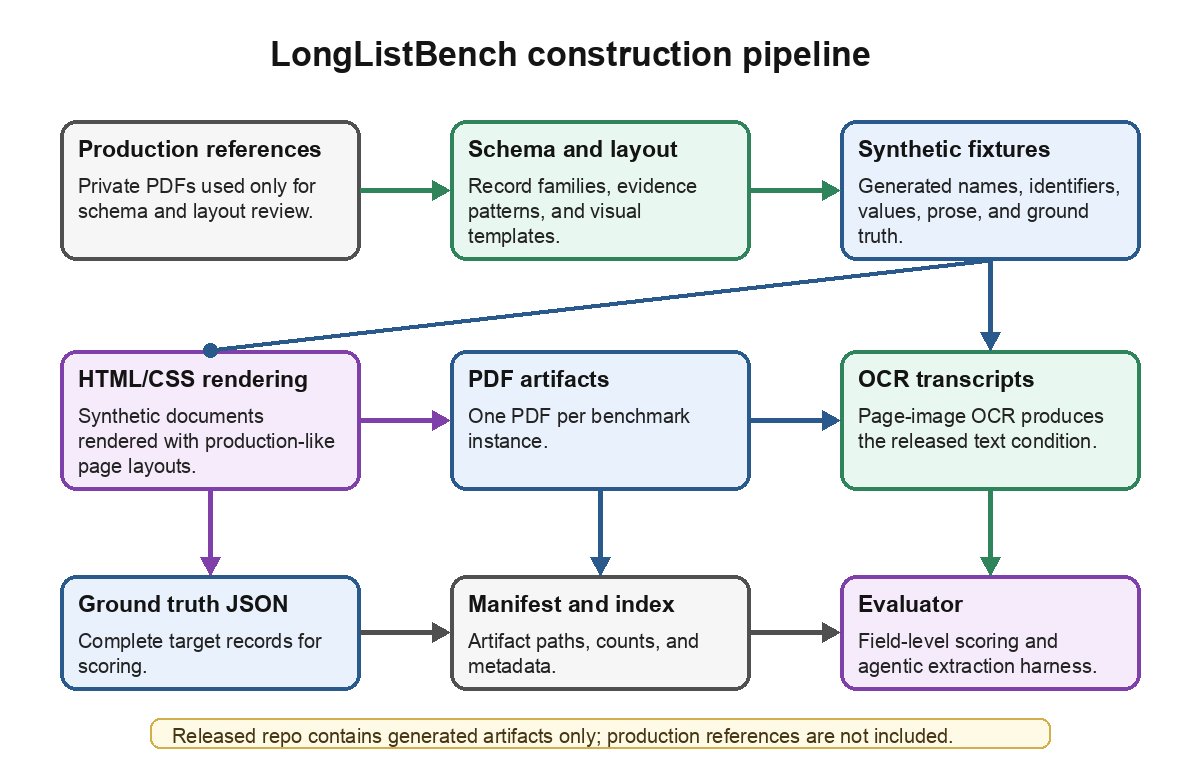
\includegraphics[width=0.7\linewidth]{figures/generation.png}
    \caption{Benchmark construction pipeline. Green path: schema design from real documents. Purple path: synthetic document generation and OCR processing.}
    \label{fig:generation-pipeline}
\end{figure}

Documents are rendered in one of two formats: (i) \textbf{Detailed}, which uses repeated incident blocks with narrative text and financial tables, or (ii) \textbf{Table}, which uses a compact tabular representation. The rendered PDFs also include synthetic packet covers, spreadsheet-like exports, portal receipts, request/response pages, and rotated scan excerpts inspired by recurring real-document layout patterns, without reusing private document content. All generation uses seeded randomness for reproducibility.

\subsection{Injected problem types}
We inject seven recurring document phenomena that complicate long-list extraction. These effects are applied at the HTML level prior to PDF rendering.

\paragraph{Page breaks.}
In real-world documents, page boundaries frequently interrupt local record context. In our detailed format, a single incident can begin on one page with identifiers and description while its financial breakdown appears on the next. In our table format, we instead insert page breaks between groups of rows and repeat table headers across the break. OCR systems typically process pages independently, producing separate text blocks that must be reassembled. Extraction models must therefore preserve continuity across pages and avoid dropping rows or misattaching continuation content.
\begin{figure}[ht]
    \centering
    \IfFileExists{figures/example_page_breaks.png}{
        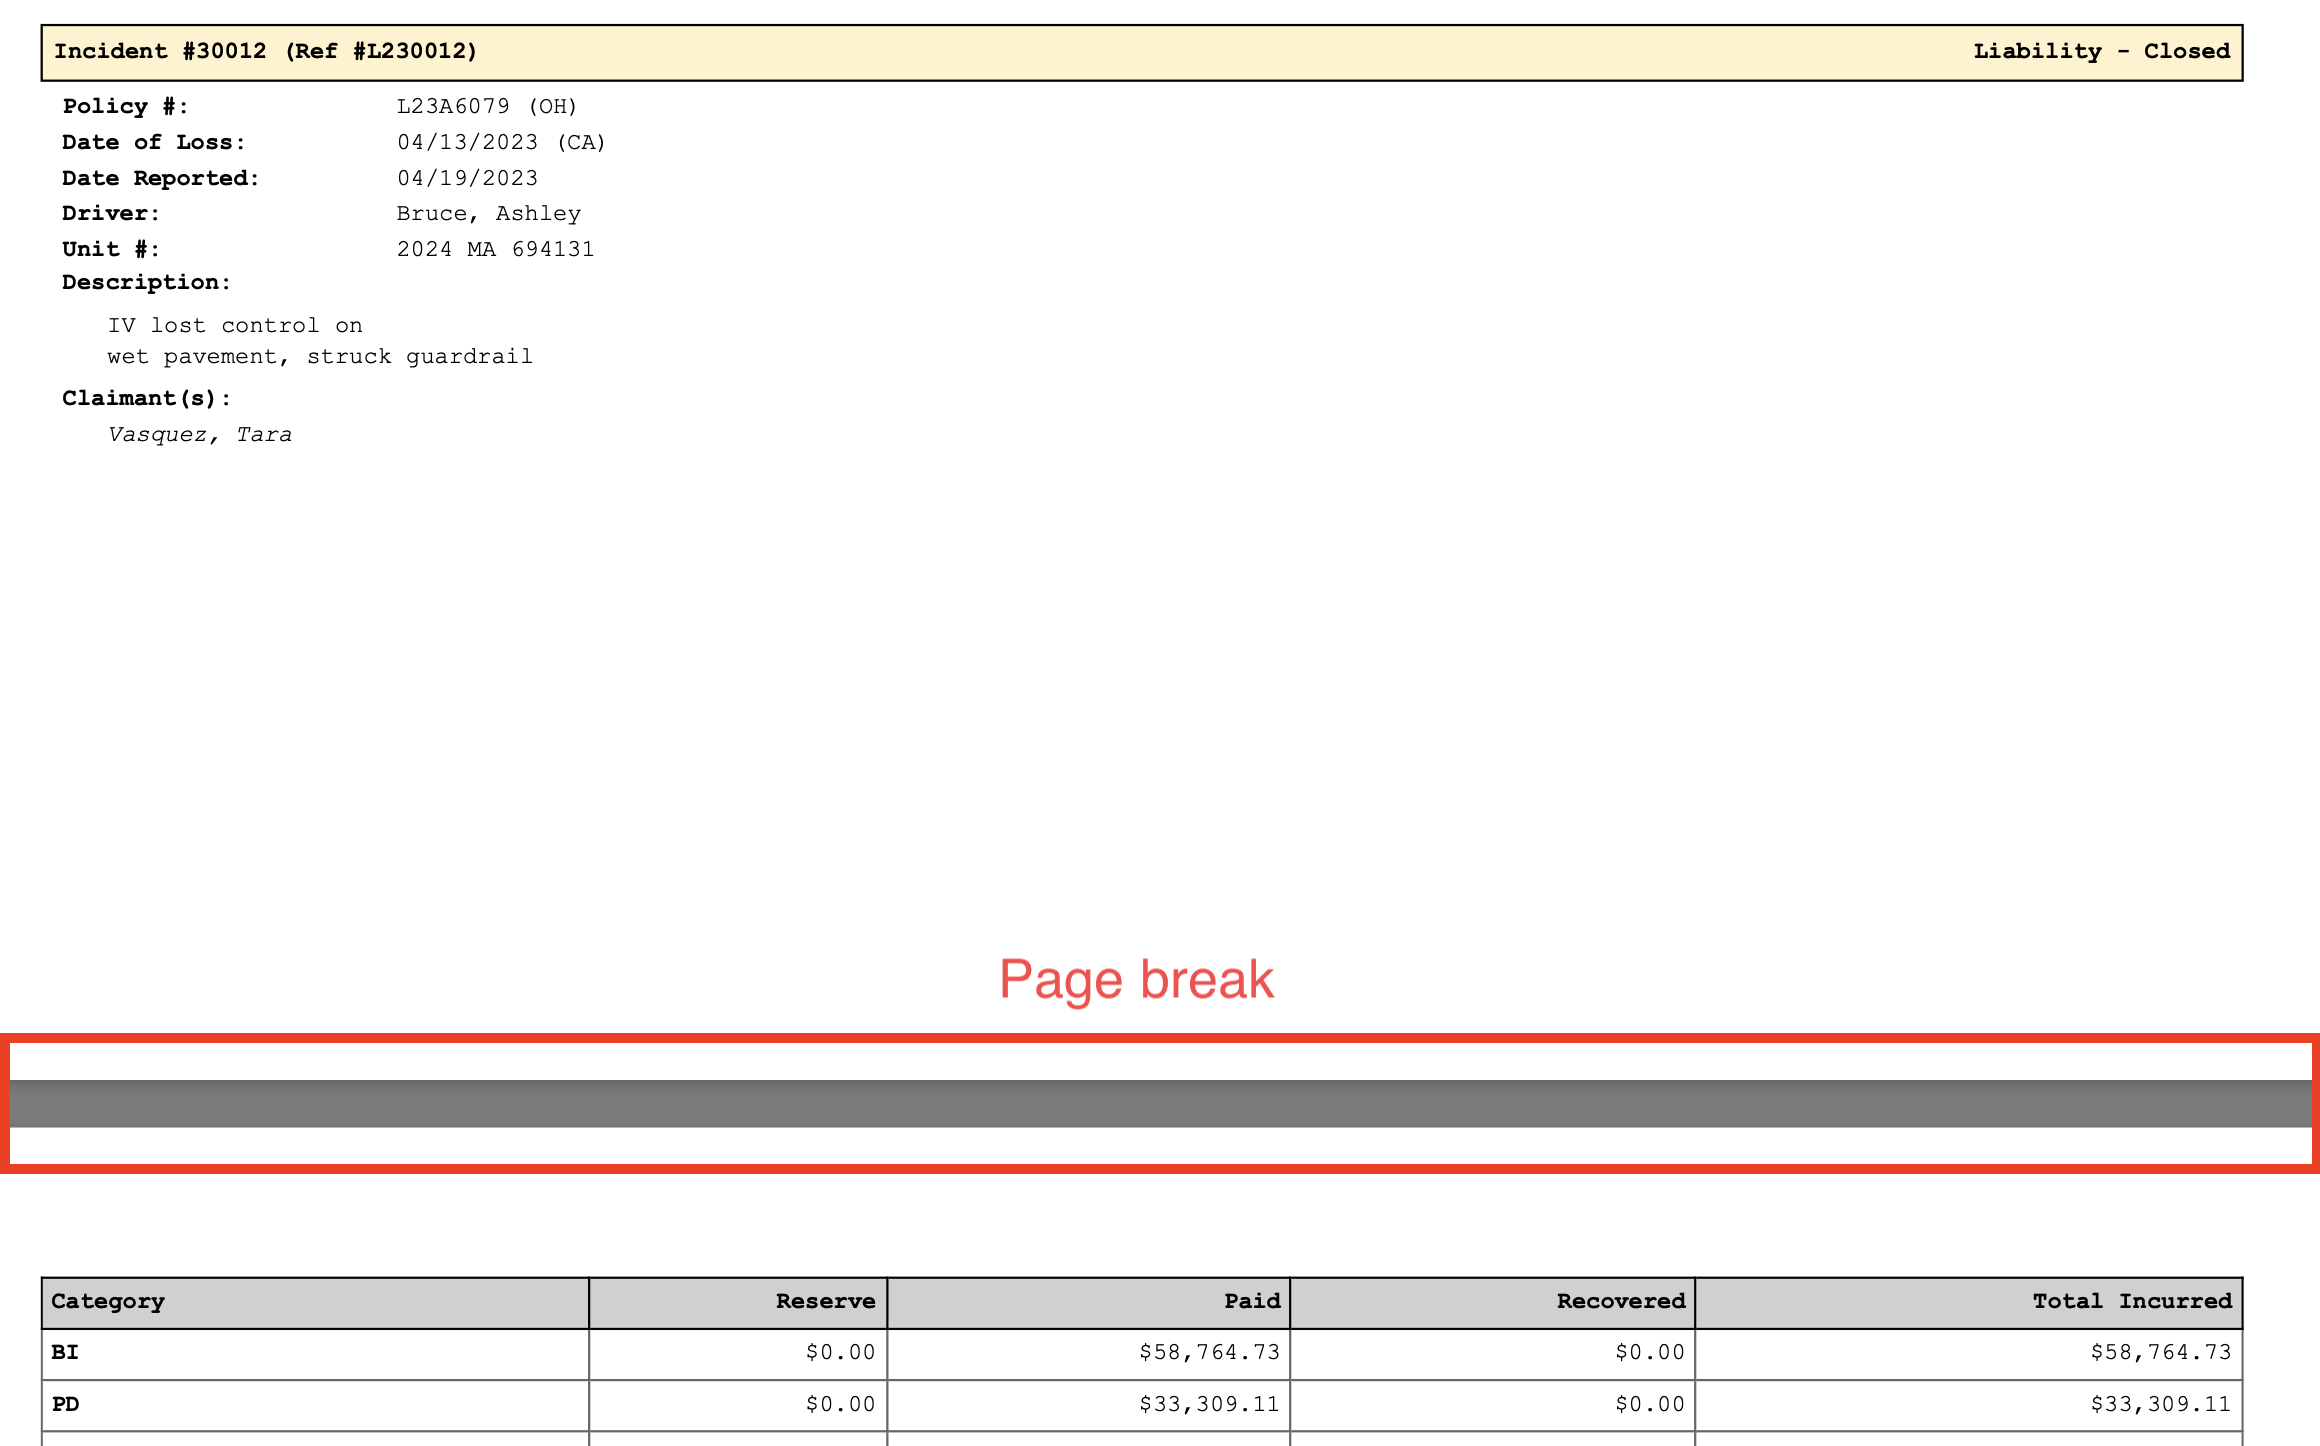
\includegraphics[width=0.95\linewidth]{figures/example_page_breaks.png}
    }{
        \fbox{\parbox{0.6\textwidth}{\centering\vspace{2cm}Page Breaks Example\vspace{2cm}}}
    }
    \caption{Example of an incident split across a page boundary.}
    \label{fig:example-page-breaks}
\end{figure}

\paragraph{Multi-row entities.}
Table cells often contain text that wraps across multiple lines, especially for description fields, addresses, or claimant lists. When OCR linearizes such content, it may interleave text from adjacent columns or treat each line as a separate cell. For example, a description spanning three lines might appear as three distinct rows in the OCR output, with column alignment lost. Extraction models must recognize that these lines belong to a single logical cell and reconstruct the original cell boundaries from visual or positional cues.
\begin{figure}[ht]
    \centering
    \IfFileExists{figures/example_multi_row.png}{
        \includegraphics[width=0.95\linewidth]{figures/example_multi_row.png}
    }{
        \fbox{\parbox{0.6\textwidth}{\centering\vspace{2cm}Multi-row Entities Example\vspace{2cm}}}
    }
    \caption{Example of a cell containing multiple lines of text.}
    \label{fig:example-multi-row}
\end{figure}

\paragraph{Exact duplicates.}
\mbox{}\\
Production documents sometimes contain intentionally repeated records. In insurance contexts, the same incident may appear multiple times due to amendments, re-openings, or reporting across multiple policy periods. Unlike data entry errors, these duplicates are semantically meaningful and must be preserved in the extracted output. Many extraction pipelines include deduplication as a post-processing step, which would incorrectly collapse valid duplicate entries. In LongListBench v1 we model this stressor as exact record repeats rather than near-duplicates or amended variants.

\paragraph{Large documents.}
Real loss runs and itemized bills routinely contain hundreds of line items. A single trucking company's annual loss run may list 200--500 incidents; a hospital bill for a complex procedure can exceed 1{,}000 charge lines. These documents push against context window limits of current LLMs. Even models with 128K+ token windows may exhibit degraded recall on items appearing in the middle of very long documents (the "lost in the middle" phenomenon). We include an extreme tier with 500 incidents per document to measure how extraction quality scales with document length.

\paragraph{Multiple tables.}
Business documents frequently embed auxiliary tables alongside the primary data. A loss run PDF might include a cover page with agent contact information, a summary table of totals by coverage type, or a glossary of status codes; none of these should be extracted as incident records. Models must distinguish the target entity table from these distractors based on schema matching, header recognition, or positional cues. Naive approaches that extract all tabular content will produce false positives from irrelevant tables.

\paragraph{Multi-column layout.}
Some documents use multi-column layouts to fit more content per page. This creates reading-order ambiguity: should text be read left-to-right across columns or top-to-bottom within each column? Standard OCR often assumes a single-column flow, interleaving content from parallel columns into an incoherent sequence. In LongListBench v1 this stressor primarily affects detailed-format primary content and auxiliary sections; the main table-format claims table remains single-span to preserve a readable tabular baseline.
\begin{figure}[ht]
    \centering
    \IfFileExists{figures/example_multi_column.png}{
        \includegraphics[width=0.95\linewidth]{figures/example_multi_column.png}
    }{
        \fbox{\parbox{0.6\textwidth}{\centering\vspace{2cm}Multi-column Layout Example\vspace{2cm}}}
    }
    \caption{Example of a two-column document layout.}
    \label{fig:example-multi-column}
\end{figure}

\paragraph{Merged cells.}
Tables often use merged cells for visual grouping. A common pattern is merging the company name cell across all incidents belonging to that company, or merging a coverage type header across its associated rows. In the rendered PDF, these appear as single cells spanning multiple rows or columns. OCR may report the merged cell's content only once, leaving subsequent rows with empty values for that field. Extraction models must propagate the merged value to all spanned rows, recognizing that an empty cell indicates inheritance from above rather than a missing value.
\begin{figure}[ht]
    \centering
    \IfFileExists{figures/example_merged_cells.png}{
        \includegraphics[width=0.95\linewidth]{figures/example_merged_cells.png}
    }{
        \fbox{\parbox{0.6\textwidth}{\centering\vspace{2cm}Merged Cells Example\vspace{2cm}}}
    }
    \caption{Example of a table with merged and spanning cells.}
    \label{fig:example-merged-cells}
\end{figure}

\subsection{Dataset scale}
The core released suite (\texttt{longlistbench-v1}, version 1.0.2) contains 80 rendered documents (40 detailed, 40 table) with 6{,}828 incident rows and canonical transcripts for evaluation. Difficulty tiers are configured as 15 easy base instances (seeded with 10 claims/PDF), 12 medium (25), 8 hard (50), and 5 extreme instances seeded with 100 claims/PDF and then expanded to 500 incidents per released document via \texttt{large\_doc}. Each base instance is rendered in both detailed and table formats, yielding 80 documents in total. Enabling \texttt{duplicates} injects additional duplicate rows, causing some documents to exceed the seed count. OCR transcripts can be generated from the rendered PDFs and should be regenerated whenever PDFs are changed.

Across the 80 documents, the most common injected issues are multi-row entities (62/80), page breaks (56/80), duplicates (56/80), and multiple tables (40/80).

\subsection{Long-range cross-page multi-hop extension}
Many production extraction tasks are not contained in one adjacent table region. A target loss-run record may require joining a front-matter claim schedule against policy registers, driver rosters, cause-code appendices, claimant indexes, and payment ledgers that appear much later in the same PDF. This pattern is awkward for one-shot extraction and naive chunking because the model must preserve join keys across large page and token distances, then merge partial records without confusing distractor rows.

To make this failure mode measurable, we add an initial multi-hop extension in the shared \path{data/} layout. It currently contains 6 single-document cross-page PDFs. Three claim-oriented cases contain 77 target incidents and use the same incident schema as the core suite; the rendered PDFs are 76, 126, and 198 pages. Three additional cases are synthetic commercial insurance policy packets: Businessowners Policy (BOP), Workers Compensation (WC), and Commercial General Liability (CGL). A policy packet is the contract document issued by an insurer; it combines declarations, covered locations or classifications, coverage limits and deductibles, rating or premium schedules, required forms, and endorsements that modify the base policy. These policy cases contain 345 target records across heterogeneous schemas for locations, coverage items, class-code or exposure items, forms, endorsements, and premiums. Each case includes one PDF, one HTML source, one \path{ground_truth} JSON file, a canonical transcript, reproducible OCR transcript generation, and per-sample metadata describing the evidence map and join requirements.

The claim-oriented extension uses the following join patterns:
\begin{itemize}
    \item \texttt{policy\_number} $\rightarrow$ policy register for company, insured, division, policy state, and agency fields.
    \item \texttt{unit\_number} $\rightarrow$ driver roster for driver identity.
    \item \texttt{cause\_code} $\rightarrow$ cause-code appendix for coverage type and normalized description.
    \item \texttt{incident\_number} $\rightarrow$ claimant index and financial ledger for claimants, adjuster notes, and nested financial breakdowns.
\end{itemize}

The policy-oriented extension adds joins such as location/building numbers to described premises, form numbers to forms-and-endorsements schedules, class codes to rating schedules, and coverage or endorsement references to distant detail pages. The largest cross-page documents mix these joins with archived distractor sections that reuse overlapping policy/reference values but contain out-of-scope records. This design is intended to stress extraction systems that can inspect long documents, preserve join keys across distant sections, and verify record completeness. The claim-oriented cases preserve comparability with the base incident schema and scorer; the policy-oriented cases use the heterogeneous record-list scorer released with the evaluation pipeline.
